%% LyX 2.3.6 created this file.  For more info, see http://www.lyx.org/.
%% Do not edit unless you really know what you are doing.
\documentclass[english]{article}
\usepackage[T1]{fontenc}
\usepackage[latin9]{inputenc}
\usepackage{graphicx}
\usepackage{babel}
\usepackage{minted}
\renewcommand{\listingscaption}{Listing}

\begin{document}
\begin{enumerate}
\item Tampilkan jumlah siswa yang ada dalam tabel siswa (point 10)

\begin{minted}{sql}
SELECT
  COUNT(nis) AS `jumlah siswa`
FROM siswa;
\end{minted}

\begin{center}
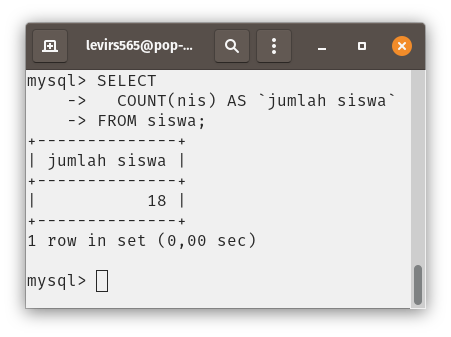
\includegraphics[scale=0.5]{1}
\par\end{center}
\item Tampilkan Jumlah penulis sebagai penerbit yang ada (point 10)

\begin{minted}{tex}
SELECT 
  COUNT(DISTINCT(penulis)) AS `penerbit yang ada` 
FROM buku;
\end{minted}

\begin{center}
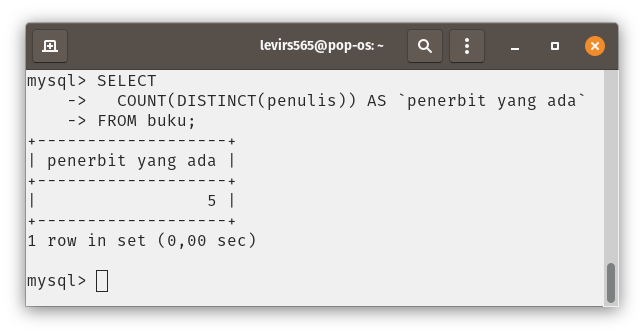
\includegraphics[scale=0.5]{2}
\par\end{center}
\item Tampilkan jumlah stock awal terbanyak sebagai stock terbanyak pada
tahun 2010 (point 10)

\begin{minted}{tex}
SELECT 
  MAX(stok_awal) AS `stock terbanyak`
FROM buku
  WHERE tahun_terbit = 2010;
\end{minted}

\begin{center}
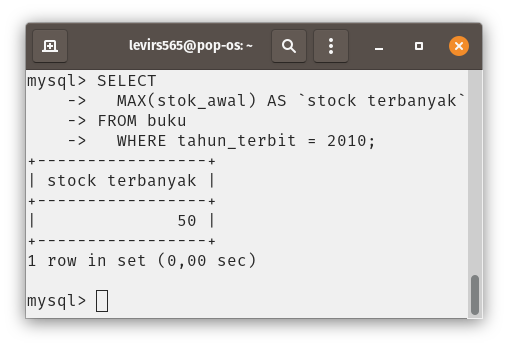
\includegraphics[scale=0.5]{3}
\par\end{center}
\item Tampilkan Jumlah kelas paling sedikit (point 10)

\begin{minted}{tex}
SELECT 
  MIN(jumlahSiswa) AS `jumlah kelas paling sedikit`
FROM (
  SELECT 
    COUNT(nis) AS jumlahSiswa
  FROM siswa
  GROUP BY kelas
) AS kelas
\end{minted}

\item Tampilkan total buku sebagai banyak buku per penulis sebagai penerbit
(point 10)

\begin{minted}{tex}
SELECT 
  penulis AS penerbit, 
  COUNT(kode_buku) AS `banyak buku` 
FROM buku 
GROUP BY penulis;
\end{minted}

\begin{center}
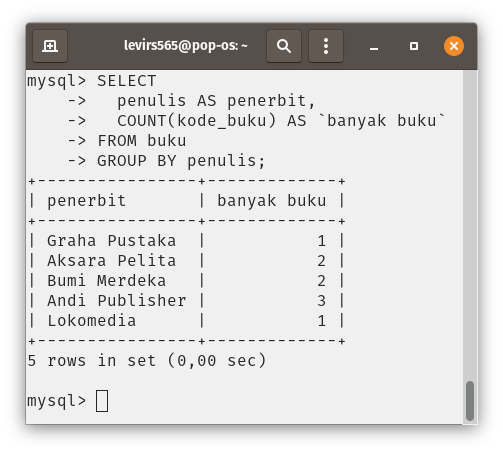
\includegraphics[scale=0.5]{5}
\par\end{center}
\item Tampilkan total judul sebagai total buku per penulis sebagai penerbit
yang lebih besar dari 1(point 20)

\begin{minted}{tex}
SELECT 
  penulis AS penerbit, 
  COUNT(judul) AS `total buku` 
FROM buku 
GROUP BY penulis
  HAVING `total buku` > 1;
\end{minted}

\begin{center}
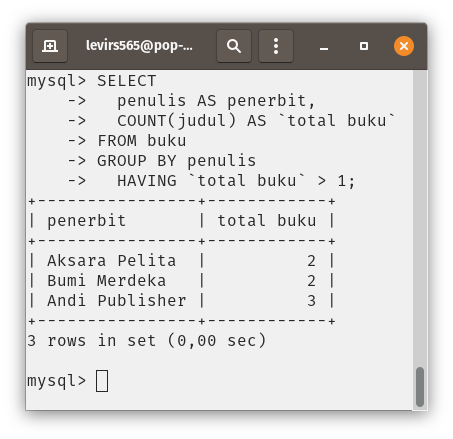
\includegraphics[scale=0.5]{6}
\par\end{center}
\item Tampilkan judul buku dan panjang karakternya diatas tahun 2009 (point
10)

\begin{minted}{tex}
SELECT
	judul,
	LENGTH(judul) AS `panjang karakter`
FROM buku
	WHERE tahun_terbit > 2009;
\end{minted}

\begin{center}
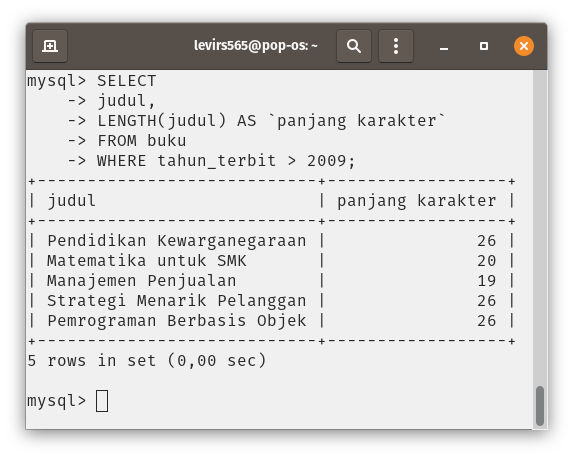
\includegraphics[scale=0.5]{7}
\par\end{center}
\item buatlah query seperti hasil dibawah ini (point 20):

\begin{minted}{tex}
SELECT
  Siswa.nis,
  Siswa.nama,
  DATE_FORMAT(
    Peminjaman.tgl_pinjam, 
    "%d %M %Y") 
  AS tanggal_pinjam
FROM siswa Siswa
  INNER JOIN peminjaman Peminjaman
    ON Peminjaman.nis = Siswa.nis
WHERE Peminjaman.tgl_pinjam >= '2012-09-27'; 
\end{minted}

\begin{center}
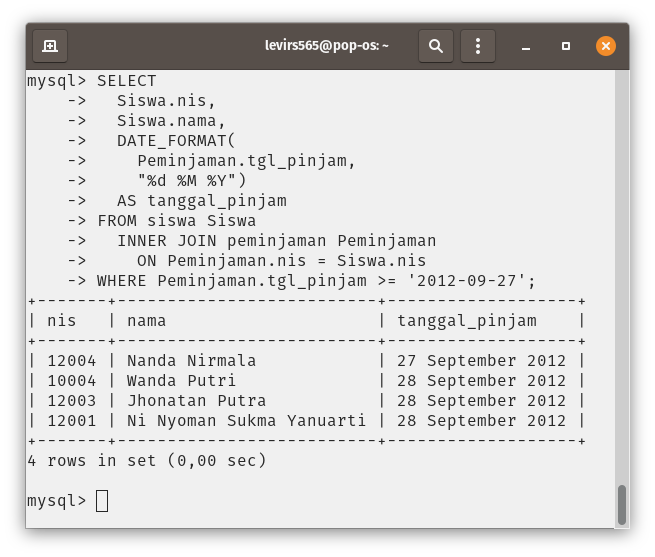
\includegraphics[scale=0.5]{8}
\par\end{center}
\end{enumerate}

\end{document}
